\documentclass[hyperref={pdfpagelabels=false},t,10pt]{beamer}
\usepackage[utf8]{inputenc}
\usepackage[english]{babel}
\usepackage[T1]{fontenc}
\usepackage[default,scale=.95]{opensans}


\usetheme[cd2018]{tud}
\setbeamercolor{normal text}{fg=black}
\colorlet{alert}{cdblue}
\setbeamercolor{alerted text}{fg=cdblue}
\setbeamerfont{frametitle}{size=\Large,family=\sffamily,series=\sbseries}


\DeclareRobustCommand\sbseries{\fontseries{sb}\selectfont}
\DeclareTextFontCommand{\textsb}{\sbseries}


\title{TITLE}
\author[© author]{Maik Thanh Nguyen}
\institute{Technische Universit\"at Dresden}
\datecity{CONFERENCE}
\date{DATE}


\begin{document}

%%%% Uncomment the following line to set background image to main slide
%%%% (parameter sets transparency)
%\setbeamertemplate{tud background}[image/shaded]{background.jpg}{0.5}
\addtocounter{framenumber}{-1}
\maketitle

\begin{frame}
  \frametitle{Content}

  \begin{itemize}
  \item Modal logic and semantics
    \begin{itemize}
        \item Kripke frames
        \item Topological space
        \item Neighbourhood frames
     \end{itemize}
  \item Multimodal logic and product of frames/spaces and logics
    \begin{itemize}
      \item Notation, Fusion of logics
      \item Horizontal and Vertical topology/functions and semantics
      \item Product of logics
    \end{itemize}
  \item Main result and ideas
  \end{itemize}
\end{frame}

\begin{frame}
  \frametitle{Modal logic and Kripke frames and models}
  \begin{itemize}
    \item Modal logic extends classical propositional logic. Formally:
    $$\phi ::= p \mid \bot \mid \neg \phi \mid \phi \lor \phi \mid \Box \phi$$
    where $\Box$ is a modal operator and Prop is a set of variable with $p \in$ Prop.
    %Other connectives are expressed through $\neg$ and $\lor$ and dual modal operator $\lozenge$ as $\lozenge \phi = \neg \Box \neg \phi$. 
     \pause

    \item A frame $F = (W,R)$ is a pair where 
    \begin{itemize}
      \item $W$ is a non-empty set of worlds
      \item $R \subseteq W \times W$ is a binary relation  
    \end{itemize}

    \item A model is a pair $M = (F,R)$ ($M$ is based on $F$) where
      \begin{itemize}
        \item $F$ is a frame
        \item $V$ is a valuation and is of the form $V : Prop \rightarrow 2^W$
      \end{itemize}
  \end{itemize}
\end{frame}

\begin{frame}
  \frametitle{Kripke semantics}
  \begin{itemize}
    \item Let $M = (F,V)$ be a model and $w \in W$ a state in $M$. A formula being true at $w$ is inductively defined as: 
  \end{itemize}

  \begin{align*}
    M, w &\Vdash p &&\text{ iff } w \in V(p) \\
    M, w &\Vdash \bot  &&\text{ never } \\
    M, w &\Vdash \neg \phi &&\text{ iff not } M, w \Vdash \phi \\ 
    M, w &\Vdash \phi \lor \psi &&\text{ iff } M,w \Vdash \phi \lor M,w \Vdash \psi \\
    M, w &\Vdash \Box \phi &&\text{ iff } \forall v \in W : wRv \rightarrow M, v \Vdash \phi \\
    M, w &\Vdash \lozenge \phi &&\text{ iff } \exists v \in W : wRv \land M,v \Vdash \phi
\end{align*}
  
\end{frame}

\begin{frame}
  \frametitle{Example}
  \begin{itemize}
    \item Let $\phi = \Box p$ and $M = (W,R,V)$ with $W = \{w_1,w_2,w_3,w_4,w_5\}$, $V(p) = \{w_3,w_4,w_5\}$ and $R = $
  \end{itemize}
  \centering
  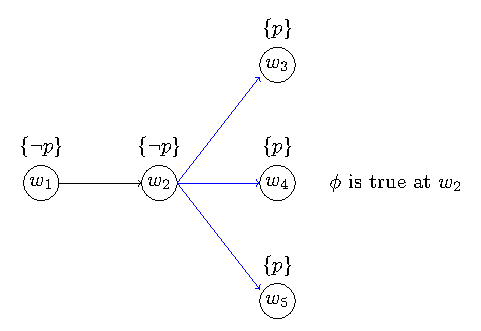
\includegraphics[width=0.55\textwidth]{Example1.pdf}
  \pause
  \begin{itemize}
    \item Kripke semantics has many applications for example epistemic logic, temporal logic,...
  \end{itemize}
\end{frame}

\end{document}
